\documentclass{vilniustech-en}
\vilniustechsetup{
    university={Vilnius Gediminas technical university},
    faculty={Faculty of Fundamental Sciences},
    cathedral={Department of Information Systems},
    workTitle={VU CYBERTHON 2023},
    workType={Writeup},
    workAuthorNames={Aurimas Šakalys, \\
        Aleksandr Prišmont, \\
        Dmitrij Linivenko, \\
        Mikas Krukauskas, \\
        Vytautas Rastenis},
    workAuthorGroup={ITSfm-22},
    workRecipient={lecturer Leonardas Marozas}
}
\addbibresource{bibliography.bib}
\VTDocumentBegin


\section{VU CYBERTHON 2023}

\textit{VU CYBERTHON} was a \textit{capture the flag} (\textit{CTF}) type of an event, organised by \textit{Vilnius University} and collaborating companies. It took place on 2023-02-25, from 09:00 until 21:00. Our team \textit{Kiberfėjos} finished 80-th, with the score of 1355 (\autoref{fig:team_standing}). During most of the CTF we went head to head with another particapating team from university, \textit{PingsWithWings}, but they beat us at during last hours of the event.

\begin{figure}[H]
\begin{center}
    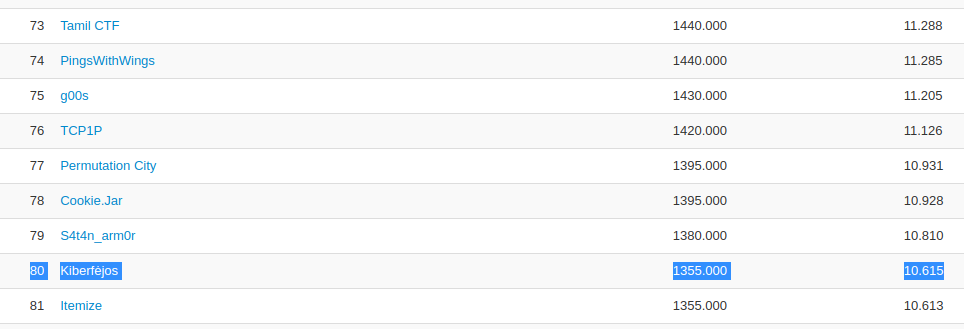
\includegraphics[width=16cm]{img/team_standing.png}
    \caption{Team standing in \textit{CTFtime}}
    \label{fig:team_standing}
\end{center}
\end{figure}

\section{Writeup}

\subsection{Forensics}

As a large portion of the tasks for the \textit{CTF} were prepared by \textit{Lietuvos teismo ekspertizės centras} \footnote{\url{https://ltec.lrv.lt/}} it had a lot of forensic tasks. The task scenario was that there was an arrest of two men near the border of Lithuania and Belarus, with a truck of weapons. A mobile phone was found. Our task was to perform forensic analysis on the binary dump of the phone file systems. 

For a large portion of the time we had used \textit{Access Data FTK Imager} that was provided to us by the organisers. Unfortunetaly, it did not contain any search functionality, and as such, most of the tasks were solved by going through the blob by hand. 

Later in the event, we were thinking of the ways that we could perform a search within the blob and decided to try to mount the existing filesystems. By creating some loop devices on the blob and later mounting the main, largest \textit{ext4} file system, we now were capable of performing search queries using \textit{unix} tools. With their help, we managed to find several additional answers in a significantly quicker way. Had we though of this technique at the start, we might have had more time to focus on unsolved tasks and perform better. We did manage to solve most of the forensic tasks, only a few of them evaded our reach (\autoref{table:solution_forensics}).

\VTTable{[
    caption = {Solution status for forensic tasks},
    label = {table:solution_forensics}
    ]{
    colspec = {X[8] X[2]},
    row{1} = {font=\bfseries}
    }
    Task & Status \\
    What is SHA1 checksum of image file blk0\_mmcblk0.bin? & Solved \\
    What is the name of the largest partition? & Solved \\
    What is the brand (vendor) of phone? & Solved \\
    What is the model of phone? & Solved \\
    What is the IMEI number of the phone? & Solved \\
    What is the SIM card number (ICCID) used on the phone? & Solved \\
    What was the subscriber's phone number (MSISDN)? & Solved \\
    What was the Bluetooth MAC Address of the device? & Solved \\
    What is a Name of device user? & Solved \\
    What is a time and date when user last login on device? & Unsolved \\
    What is a Username of telegram messenger? & Solved \\
    What email address is setup on com.android.email service? & Solved \\
    Find the contact related to Belarus? & Unsolved \\
    Find the contact related to Russia? & Solved \\
    What is a name of video file which is related with tanks? & Solved \\
    What is a name of audio file which is related with rifles and... & Solved \\
    Based on the review of the media files, please provide the GPS... & Solved \\
    What tank specs the user was looking for? & Solved \\
    What date and time this search was performed? & Unsolved \\
    What is the name of WhatsApp user which has phone number... & Solved \\
    What web address was provided for a company that can rent... & Solved \\
    How much dollars the seized weapons (stuff) may have cost? & Solved \\
    Based on the analysis of the video file 20221015\_173902.mp4... & Solved \\
}

\subsection{Non-forensic tasks} 

We shall describe the rest of the tasks that were solved or attempted individually, and what kind of techniques were used to achieve the results.

\subsubsection{Challenge - Firewall}

This challenge could have possibly been much more difficult. We were provided with a binary and readable representation of the rules for \textit{Windows Firewall}. We simply loaded the rules in a \textit{Windows} virtual machine and looked over the rules. We noticed that one of the first rules seemed to be a bit out of place, and opening it, we found a \textit{base64} encoded string, which decoded into the flag.

\subsubsection{Music assignment}

In this challenge, we were provided with a copy of the main Cyberthon web page \textit{html}. Looking over it, we would find a link that would lead us to an audio file, which had morse code. By using a morse code decoder, we got the flag.

\subsubsection{Network Attack}

We were given \textit{NetFlow} and had to analyse it to determine what type of \textit{CVE} was used in the attack. The \textit{CVE} used was \textit{CVE-2020-0610}.

\subsubsection{Simple Web}

We were given an \textit{html} file. After opening it, one thing immedeately popped out - the instructions for the \textit{brainfuck} language. After putting the instructions into an \textit{brainfuck} interpreter, we would get the flag.

\subsubsection{Weak Password}

This was a frustrating task. We had been provided with a zip file, that was password locked. We were given a hint, that the password was one of the most popular password that the task creators had indicated. We've looked over a multitude of password lists, employed password cracking software, but none of the passwords worked. Even the passwords that were found by using the password cracking software did not work.  We did not manage to solve this task.

\subsubsection{Reverse Me (easy)}

We have attempted to crack this task, as it did seem to be pretty easy. By running the program we saw that it required us to enter a username and password. We put the binary into \textit{ghidra} and looked where these functions were called (\autoref{fig:reversing}). As we can see in the picture, the success path if reached when a comparison with \textit{local\_18} and \textit{local\_14} variables is performed. Here we thought that the values that were in those local variables were pointers to \textit{C} strings, which was an incorrect assumption. After looking over some of the other write-ups, we saw that the values we were supposed to enter were those values in decimal, as it was a direct integer comparison, as opposed to \textit{C} string comparison.

\begin{figure}[H]
\begin{center}
    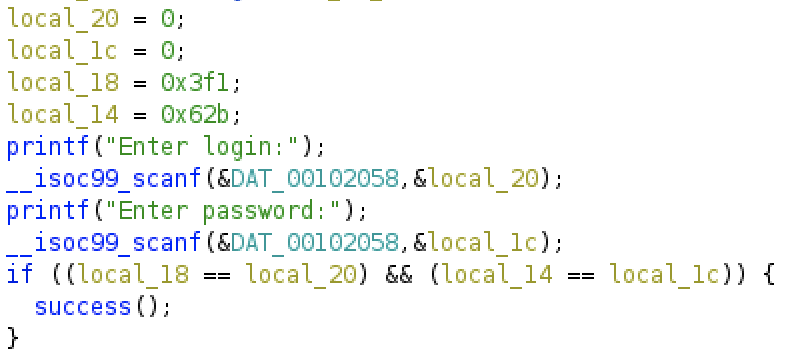
\includegraphics[width=12cm]{img/reversing.png}
    \caption{Decompiled binary}
    \label{fig:reversing}
\end{center}
\end{figure}


\subsubsection{Blue Baby Shark}

We were provided with a packet dump and we had to find the flag within the dump. By simply selecting to go through the \textit{TCP} conversation in order in \textit{Wireshark} we got back to the root of the packets and found the flag there.

\subsubsection{Find location}

We were provided with a picture. The flag was hidden in the \textit{Exif} information.

\subsubsection{Authors mistake}

We were provide with a link to a \textit{Pinterest} post page. By going to the author page of the provided post and looking around, the flag was found in the comment of one of the authors \textit{Pinterest} posts (\autoref{fig:pinterest}).

\begin{figure}[H]
\begin{center}
    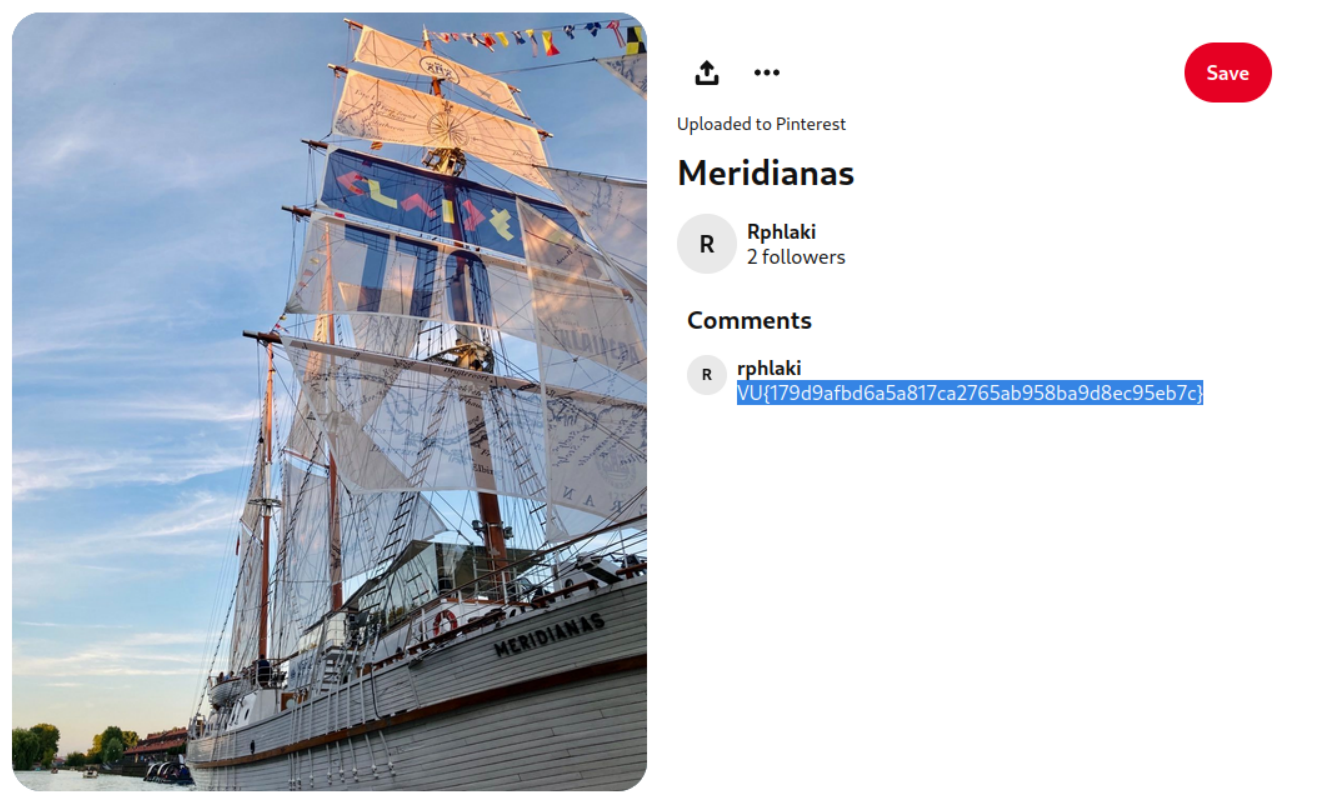
\includegraphics[width=12cm]{img/pinterest.png}
    \caption{Flag in a comment of a \textit{Pinterest} post}
    \label{fig:pinterest}
\end{center}
\end{figure}

\subsubsection{Plain sight}

Another frustrating task - we were provided with the information that dean of Vilnius University Kaunas faculty had hidden the flag in plain sight. We found the flag (\autoref{fig:windings}) on his \textit{Facebook} page, but it was encoded in a \textit{Windings} type of font. We identified that the font used was \textit{Windings 2} and recreated the message, but the flag did not work. We tried switching some of the symbols that seemed similar, but to no avail. We did not solve this task.

\begin{figure}[H]
\begin{center}
    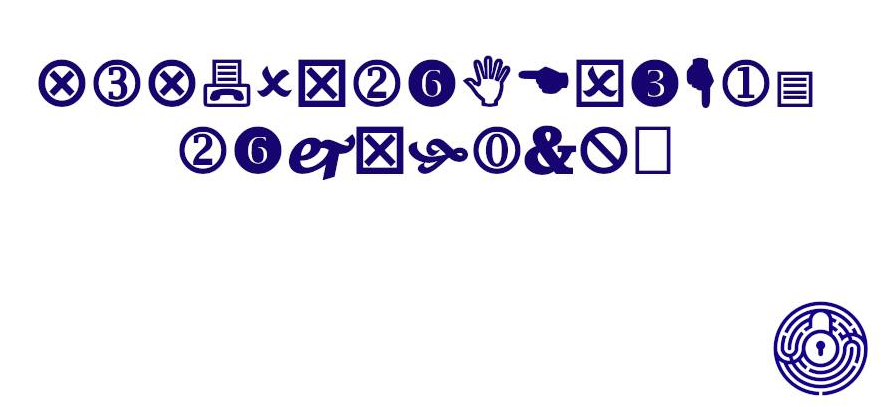
\includegraphics[width=12cm]{img/windings.png}
    \caption{Flag encoded in \textit{Windings 2} font}
    \label{fig:windings}
\end{center}
\end{figure}

\subsubsection{RFC standard for security policy information}

We were tasked to find security audit information of the \textit{Altacom} company, that uses some \textit{RFC} standard to present such audit information. This standard is \textit{RFC 8615} \footnote{\url{https://www.rfc-editor.org/rfc/rfc8615}} where web resources put certain resources under the \textit{/.well-known/} path. Additionally, \textit{RFC 9116} \footnote{\url{https://www.rfc-editor.org/rfc/rfc9116}} describes a standard of storing security vulnerability disclosure information. It is stored at \textit{/.well-known/security.txt} path. As such, if we visit \url{https://www.altacom.eu/.well-known/security.txt}, the flag is the email address to report security vulnerabilities. 

\section{Summary}

The event was fun and we have learned quite a few things about how forensics are performed, that our phones collect an awful lot of data about us. Some of the non-forensic tasks were interesting, albeit a bit simple, and some were generally weak from the presentation side. Overall, the experience was good.

\VTDocumentEnd